%%%%%%%%%%%%%%%%%%%%%%%%%%%%%%%%%%%%%%%%%%%%%%%%%%%%%%%%%%%%%%%%%%%%%%%%%%%%%%%%%%%%%%
%  File 51_advance_use.tex
%%%%%%%%%%%%%%%%%%%%%%%%%%%%%%%%%%%%%%%%%%%%%%%%%%%%%%%%%%%%%%%%%%%%%%%%%%%%%%%%%%%%%%

\section{実験設定の詳細} \label{sec:adv_settings}
%====================================================================================

ここではチュートリアルで触れなかった実験設定の詳細について説明する。SCALEでサポートする全てを
網羅してはいないが、格子間隔、計算領域、積分時間間隔、物理過程等の重要な設定方法については
できる限り丁寧に説明するように心がけた。実験設定は全て、\verb|pp_***.conf|、\verb|init_***.conf|、
および\verb|run_***.conf|のconfigファイルを編集することで設定できる。従って、以降の説明は
全てconfigファイルの編集方法について述べたものである。configファイルの設定変数の詳細は
付録\ref{app:namelist}に記載があるので、本節と併せて読み進めて欲しい。
また以下の説明は、第3章と第4章のチュートリアルをすでに実行してきたものとして説明する。


\subsection{格子間隔} \label{sec:adv_gridspace}
%------------------------------------------------------
はじめに、この設定を行う上で注意しなければならない点を挙げる。以下で説明する
\textcolor{red}{\bf 格子間隔の設定は、pp\_***.conf、init\_***.conf、run\_***.confの
configファイルの間で必ず一致させなければならない。}このことに注意して設定変更を進めてもらいたい。

SCALEでは、格子点の位置を均等間隔で設定することも、任意の格子点位置を直接指定することもできる。
均等間隔で設定する場合は、configファイルの\verb|PARAM_GRID|の\verb|DX|、\verb|DY|、\verb|DZ|の変数を
指定することで、格子間隔を指定できる(\verb|DX|、\verb|DY|、\verb|DZ|はそれぞれ、東西、南北、鉛直方向の
格子間隔を意味する)。一方、直接格子点の位置を指定する場合は、\verb|FZ|
\footnote{SCALEの格子系はArakawa-Cグリッド、およびLorenzグリッドであるため、水平方向と鉛直方向ともに
スタッガード点(1/2ずれた点)に位置する変数がある。コントロールボリュームに対して中心点に位置する格子点を
Center Pointと呼び、コントロールボリュームの面に位置する格子点(Center Pointに対して1/2ずれている)を
Face Pointと呼ぶ。そして、これらの頭文字と方向を組み合わせてCX、CY、CZやFX、FY、FZと呼ぶ。}
などの格子点位置変数に対して直接に値を代入する。これらの変数は全て、倍精度浮動小数点変数で単位はメートル[m]である。

例として理想実験のチュートリアルのrun.confファイル(run\_R20kmDX500m.conf)を見てみると次のように記載されている。\\

\noindent {\small {\gt
\ovalbox{
\begin{tabularx}{140mm}{l}
\verb|&PARAM_GRID|\\
\verb| DX = 500.D0,|\\
\verb| DY = 500.D0,|\\
\verb| FZ(:) = |\\
\verb|    80.000000000000000      ,|\\
\verb|    168.00000190734863      ,|\\
\verb|    264.80000610351567      ,|\\
\verb|     〜 中略 〜|\\
\verb|    14910.428862936289      ,|\\
\verb|    15517.262523292475      ,|\\
\verb|    16215.121232702089      ,|\\
\verb|    17017.658748523147      ,|\\
\verb|    17940.576891717363      ,|\\
\verb|    19001.932756390710      ,|\\
\verb|    20222.492000765058      ,|\\
\verb| BUFFER_DZ = 5000.D0,|\\
\verb| BUFFFACT  =   1.0D0,|\\
\verb|/|\\
\end{tabularx}
}}}\\

\verb|DX|、\verb|DY|は``\verb|500.D0|''と倍精度表記を用いて500 mと指定されており、水平方向の格子間隔は
500 mの均等間隔に設定されていることがわかる。例えば、2 kmの格子間隔で実験がしたければ、
ここに``\verb|2000.D0|''と記述すればよい。

一方、\verb|FX(:)|の項目は鉛直方向の格子点位置を直接指定している。ここには示していないが、同じconfigファイル中の
\verb|PARAM_INDEX|の項目に``\verb|KMAX = 97|''として鉛直97層であると設定されているため、最下層から再上層まで
97層分の位置が指定されている。これを見れば、最下層の高度は80 m、最上層の高度は約20 kmであるとわかる。
モデルの鉛直層とり方を変えたい場合は、これに習って\verb|KMAX|で指定した層数に応じて高度をしていすればよい
\footnote{独自の鉛直層設定の作成をサポートするツールとして、scale/scale-rm/util/makevgridのディレクトリ下に
``make\_vgrid.f90''というFortranプログラムといくつかのサンプルnamelistが用意されている。これをコンパイルして
実行すれば直ちにconfigファイルに貼り付けて使用できるフォーマットになった鉛直層設定を作成できる。}
。


\subsubsection{バッファー格子点の設定}

SCALEでは計算領域境界のすぐ内側に「バッファー格子点」を設定することができる。バッファー格子点では、指定された値や
親モデルのデータにダンピングする、いわゆるナッジングが行われる。これは、モデル最上層で重力波が反射することを
緩和するための「スポンジ層」として利用したり、現実大気実験を行う際に側面境界において親モデルと
SCALEで計算される大気場が乖離することを防ぐための「緩和領域」として利用される。

バッファー格子点は、\verb|BUFFER_DX|、\verb|BUFFER_DY|、\verb|BUFFER_DZ|、および\verb|BUFFFACT|の変数によって
設定される。\verb|BUFFER_DX|、\verb|BUFFER_DY|、\verb|BUFFER_DZ|は、それぞれの方向のバッファー領域の幅
(単位はメートル)を示す。バッファー領域は境界から内側に\verb|BUFFER_DX|等で指定された幅で設置され、
バッファー領域内の格子点はバッファー格子点として認識される。したがって、その分だけナッジングの影響を受けないで計算
される自由領域は狭くなることに注意が必要である。水平方向には東西南北どの方向にも同様にバッファー領域が設定されるが、
鉛直方向には計算領域の上端にのみバッファー領域が設定され、下端には設定されない。
\verb|BUFFFACT|はバッファー領域内の格子点の格子間隔に対するストレッチ係数である。
下記の関係式によって、バッファー領域内の格子間隔(BDX)は決定される。
\begin{eqnarray}
BDX_{i+1}={BDX_{i}}^{BUFFFACT} \nonumber \\
BDX_{1}=DX_{default} \nonumber
\end{eqnarray}
ここで、$i$はバッファー領域内の格子点番号を表し、計算領域の内側から外側へ向かって番号が振られる。
$DX_{default}$は\verb|PARAM_GRID|の項目で設定される元々の\verb|DX|を意味する。
$i$の最大値$ni$は、$\sum_{i=1}^ni BDX_{i} > BUFFER_{DX}$の関係を達成する最小の数として決定される。
したがって、``\verb|BUFFFACT = 1.0|''ならば、格子間隔をストレッチせずに等間隔であることを意味し、
``\verb|BUFFFACT = 1.2|''ならば、計算領域の内側から境界へ向けて、格子点間距離がもともとの格子間隔から
1.2倍の割合で広がっていくことを意味する。\verb|BUFFFACT|の値を大きくすると、バッファー領域の幅が同じでも
バッファー格子点として使用される格子点数は少なくなる。

例として理想実験のチュートリアルのrun.confファイル(run\_R20kmDX500m.conf;上に表示したもの)を見てみると、
\verb|BUFFER_DZ = 5000.D0|、\verb|BUFFFACT = 1.0D0|と指定されている。\verb|BUFFER_DZ|以外には指定がないので、
水平方向にはバッファー領域が設定されない(この実験は水平方向には周期境界条件になっておりバッファー領域は必要ない)。
\verb|BUFFFACT = 1.0D0|となっているため、もとの格子間隔のままストレッチは行わない。
最上層の高度が20222 mと指定されており、鉛直方向のバッファー領域の幅は5000 mと指定されているため、
モデル計算領域のトップから高度15222 mまでがバッファー領域となる。鉛直層の高度指定によれば、92層目の高度が
15517 mで、91層目の高度が14910 mであるため、92層目まではバッファー領域だが、91層目はバッファー領域ではない。
繰り返しになるが、これらの設定は\verb|pp_***.conf|、\verb|init_***.conf|、\verb|run_***.conf|の
すべてのconfigファイルにおいて共通した設定になっていなければならない。

SCALEでは、バッファー領域の大きさ、バッファー格子点の数について、まだ明確な指標を設定できていないが、
鉛直方向(計算領域トップ)のバッファー格子点は5点以上、水平方向(側面境界付近)のバッファー格子点は
20〜40点程度を推奨している。実験設定や事例によっては、さらにバッファー格子点を増やしたり、ストレッチ係数を
用いてバッファー領域を広げる処理が必要であったり、ここでは説明しなかったが\verb|ATMOS_BOUNDARY_taux|、
\verb|ATMOS_BOUNDARY_tauy|といった設定項目を調整してバッファー領域のナッジング強度を強める必要があったりする。



\subsection{計算領域の大きさ} \label{sec:adv_domainsize}
%------------------------------------------------------
ここで説明する\textcolor{red}{\bf 計算領域の設定は、pp\_***.conf、init\_***.conf、run\_***.confの
configファイルの間で必ず一致させなければならない。}このことに注意して設定変更を進めてもらいたい。

SCALEはMPI並列プログラムであり、全計算領域は複数のMPIプロセスに分割されて並列実行される。計算領域は
水平2次元(東西方向 $\times$ 南北方向)に分割される。したがって計算領域の大きさは、MPIプロセス数と
1つのMPIプロセスが担当する格子点数によって決まる。以降、X方向は水平軸の東西方向、Y方向は水平軸の南北方向を
それぞれ意味するものとする。

X方向、およびY方向のMPIプロセスの割付設定は、configファイルの\verb|PARAM_PRC|の項目にある\verb|PRC_NUM_X|、
および\verb|PRC_NUM_Y|よって指定される。また、1つのMPIプロセスが担当する格子点数は、
\verb|PARAM_INDEX|項目にある\verb|KMAX|、\verb|IMAX|、\verb|JMAX|の変数によって指定され、
それぞれ鉛直方向、X方向、Y方向の格子点数を表す。
したがって、X方向の総格子点数は\verb|PRC_NUM_X| $\times$ \verb|IMAX|、Y方向の総格子点数は
\verb|PRC_NUM_Y| $\times$ \verb|JMAX|と表現される。また、計算に必要な総MPIプロセス数は、
\verb|PRC_NUM_X| $\times$ \verb|PRC_NUM_Y|となる。実行時にMPIコマンドに指定するMPIプロセス数は、
この総MPIプロセス数を指定しなければならない。この条件を満たさない場合は,LOGファイルなどに\\

\noindent {\small {\gt
\ovalbox{
\begin{tabularx}{140mm}{l}
\verb|xxx total number of node does not match that requested. Check!| \\
\end{tabularx}
}}}\\

\noindent というメッセージが出力がされて計算が異常終了するので、設定、もしくは実行コマンドを見なおしてもらいたい。

ここまでの復習として、現実大気実験のチュートリアルで使用した\verb|run.conf|ファイルを例にして、
上述の内容を確認してみる。\\

\noindent {\small {\gt
\ovalbox{
\begin{tabularx}{140mm}{l}
\verb|&PARAM_PRC| \\
\verb| PRC_NUM_X      = 2,| \\
\verb| PRC_NUM_Y      = 2,| \\
\verb| PRC_PERIODIC_X = .false.,| \\
\verb| PRC_PERIODIC_Y = .false.,| \\
\verb|/| \\
 \\
\verb|&PARAM_INDEX| \\
\verb| KMAX = 36,| \\
\verb| IMAX = 60,| \\
\verb| JMAX = 60,| \\
\verb|/| \\
\end{tabularx}
}}}\\

\noindent まずMPIプロセス数については\verb|PRC_NUM_X = 2|、\verb|PRC_NUM_Y = 2|と設定されているため、
X方向、Y方向ともに2分割されており、総計として4つのMPIプロセスを使用した計算となることがわかる。
一方、1つのMPIプロセスあたりの格子点数については、\verb|IMAX = 30|、\verb|JMAX = 30|と指定されているため、
総格子点数としては、X方向、Y方向ともに$2 \times 60 = 120$となり120格子点である。
同じconfigファイル内に記載されている\verb|PARAM_GRID|の項目の\verb|DX|、\verb|DY|はともに15000 m(15 km)
と指定されているため、$120 grid \times 15 km = 1800 km$の計算から、$1800 km \times 1800 km$の正方形の計算領域
が設定されていることがわかる。

\verb|PARAM_PRC|の項目の\verb|PRC_PERIODIC_X|、\verb|PRC_PERIODIC_Y|は側面境界条件に関する設定である。
その詳細は次節で説明する。


\subsubsection{計算領域の変更例}
ここでは、現実大気実験のチュートリアルのconfigファイル(\verb|run.conf|)を元にしていくつかの変更例を説明する。
以下の変更例をもとに、自分の行いたい実験設定にあったconfigファイルを作り上げてもらいたい。\\


{\bf a. MPIプロセス数はそのままに計算領域を4倍に広げる}\\

この設定はとても簡単である。デフォルト設定は、X方向、Y方向ともに2つのMPIプロセスを使用し、格子点数はともに
30点なので、全領域の格子点数は、$(2 \times 60)_{x} \times (2 \times 60)_{y} = 14400$点である。
従って、計算領域を4倍に広げるためには、\verb|IMAX|、\verb|JMAX|の値をデフォルトに対して2倍の値に変更するだけである。
これで、全領域の格子点数は、$(2 \times 120)_{x} \times (2 \times 120)_{y} = 57600$点となり、14400点の4倍の
計算領域になっている。この変更を施したconfigファイルの例は次のとおりである。
赤文字の部分がデフォルトからの変更点を意味する。\\

\noindent {\small {\gt
\ovalbox{
\begin{tabularx}{140mm}{l}
\verb|&PARAM_PRC| \\
\verb| PRC_NUM_X      = 2,| \\
\verb| PRC_NUM_Y      = 2,| \\
\verb| PRC_PERIODIC_X = .false.,| \\
\verb| PRC_PERIODIC_Y = .false.,| \\
\verb|/| \\
 \\
\verb|&PARAM_INDEX| \\
\verb| KMAX = 36,| \\
\textcolor{red}{\verb| IMAX = 120,|} \\
\textcolor{red}{\verb| JMAX = 120,|} \\
\verb|/| \\
\end{tabularx}
}}}\\

\vspace{5mm}
{\bf b. 1つのMPIプロセスあたりの格子点数はそのままに計算領域を4倍に広げる}\\

先程は、MPIプロセス数を維持して計算領域を広げたが今度は、1つのMPIプロセスあたりの格子点数はそのままに、MPIプロセス数を
増やすことで計算領域を4倍に広げる方法を説明する。1つのMPIプロセスあたりの格子点数(プロセスあたりの演算量)は
そのままにMPIプロセス数を増やすことで計算領域を広げる(総演算量を増やす)。この場合、1つのCPUが担当する問題サイズは
変わらないため、理想的には計算にかかる時間を増やすことなく計算領域を広げることができる
\footnote{計算科学用語では、この変更、つまりプロセスあたりの演算量一定で総演算量を増やしていくことを``weak scaling''と呼ぶ。}。

計算領域を4倍に広げるためには、\verb|PRC_NUM_X|、\verb|PRC_NUM_Y|の値をデフォルトに対して2倍の値に変更するだけである。
これで、全領域の格子点数は、$(4 \times 60)_{x} \times (4 \times 60)_{y} = 57600$点となり、14400点の4倍の
計算領域になっている。このとき必要なMPIプロセス数は、$4 \times 4 = 16$プロセス、つまりデフォルトの4倍のMPIプロセス数が必要になる。
この変更を施したconfigファイルの例は次のとおりである。赤文字の部分がデフォルトからの変更点を意味する。\\

\noindent {\small {\gt
\ovalbox{
\begin{tabularx}{140mm}{l}
\verb|&PARAM_PRC| \\
\textcolor{red}{\verb| PRC_NUM_X      = 4,|} \\
\textcolor{red}{\verb| PRC_NUM_Y      = 4,|} \\
\verb| PRC_PERIODIC_X = .false.,| \\
\verb| PRC_PERIODIC_Y = .false.,| \\
\verb|/| \\
 \\
\verb|&PARAM_INDEX| \\
\verb| KMAX = 36,| \\
\verb| IMAX = 60,| \\
\verb| JMAX = 60,| \\
\verb|/| \\
\end{tabularx}
}}}\\

\vspace{5mm}
{\bf c. 計算領域はそのままに水平格子間隔を3 kmに変更する}\\

現実大気実験チュートリアルのデフォルト設定は、X方向、Y方向の総格子点数は120点で水平格子間隔が15 kmなので、
計算領域は1800 km $\times$ 1800 kmの領域となっている。ここでは、この領域を維持したまま水平格子間隔を3 kmに
狭める設定にトライする。水平格子間隔が15 kmから3 kmへ1/5だけ小さくなるので逆に1方向あたりの総格子点数は5倍、
つまり600点必要になる。この600点をどのようにMPIプロセス数とプロセスあたりの格子点数として割り振るかは
ユーザーの環境や計算機リソース量によって異なる。たとえば、X方向、Y方向ともに10プロセスずつ、合計で100プロセスを
使えば、プロセスあたりの格子点数は60点となり、積分時間間隔が短くなることを無視すれば演算量はデフォルトと変わらない。

しかし、なかなか100プロセスを利用できる計算機を持っている環境にいる人は少ないだろう。そこで、デフォルトから
各方向に1つずつMPIプロセス数を増やし、$3 \times 3 = 9$プロセスを利用した設定を考えてみる。
1方向あたりの総格子点数は600点なので、プロセスあたりの格子点数は$600 \div 3 = 200$点となる。

ここでの変更で気をつけなければならないことは、バッファー領域の幅である。現実大気実験チュートリアルの
デフォルト設定ではバッファー領域は、計算領域トップと東西南北の側面境界に設定されており、側面境界のバッファー領域の
幅は片側300 km、つまり15 km格子間隔で20点のバッファー格子点が確保されている。水平格子間隔を15 kmから3 kmへ変更
したので、このままでは100点もの格子点がバッファー領域に取られてしまう。SCALEでは一般的に20〜40点程度の
バッファー格子点を設定するようにしているので、デフォルトと同じ20点になるように側面境界のバッファー領域の
幅は片側60 kmと設定する。鉛直層設定は変更していないため、計算領域トップのバッファー領域については設定を変更する
必要はない。

この変更を施したconfigファイルの例は次のとおりである。赤文字の部分がデフォルトからの変更点を意味する。\\

\noindent {\small {\gt
\ovalbox{
\begin{tabularx}{140mm}{l}
\verb|&PARAM_PRC| \\
\textcolor{red}{\verb| PRC_NUM_X      = 3,|} \\
\textcolor{red}{\verb| PRC_NUM_Y      = 3,|} \\
\verb| PRC_PERIODIC_X = .false.,| \\
\verb| PRC_PERIODIC_Y = .false.,| \\
\verb|/| \\
 \\
\verb|&PARAM_INDEX| \\
\verb| KMAX = 36,| \\
\textcolor{red}{\verb| IMAX = 200,|} \\
\textcolor{red}{\verb| JMAX = 200,|} \\
\verb|/| \\
 \\
\verb|&PARAM_GRID| \\
\textcolor{red}{\verb| DX = 3000.D0,|} \\
\textcolor{red}{\verb| DY = 3000.D0,|} \\
\verb| FZ(:) =    80.841D0,   248.821D0, ... ... 1062.158D0,| \\
\verb|            1306.565D0,  1570.008D0, ... ... 2845.575D0,| \\
\verb|       〜 中略 〜|\\
\verb|           18387.010D0, 19980.750D0, ... ... 28113.205D0,| \\
\verb| BUFFER_DZ = 5000.D0,| \\
\textcolor{red}{\verb| BUFFER_DX = 60000.D0,   ! 20 buffer|} \\
\textcolor{red}{\verb| BUFFER_DY = 60000.D0,   ! 20 buffer|} \\
\verb|/| \\
\end{tabularx}
}}}\\


\subsection{地図投影法と計算領域の位置} \label{sec:adv_mapproj}
%------------------------------------------------------
計算領域の位置と投影法は、configファイルの\verb|PARAM_MAPPROJ|の項目を編集することで設定できる。
\textcolor{red}{\bf この設定も、pp\_***.conf、init\_***.conf、run\_***.confのconfigファイルの間で
必ず一致させなければならない。}はじめに下記の例をもとに説明する。\\

\noindent {\small {\gt
\ovalbox{
\begin{tabularx}{140mm}{l}
\verb|&PARAM_MAPPROJ| \\
\verb| MPRJ_basepoint_lon = 138.727778D0,| \\
\verb| MPRJ_basepoint_lat = 35.360556D0,| \\
\verb| MPRJ_type          = 'MER',| \\
\verb|/| \\
\end{tabularx}
}}}\\

\noindent まず\verb|MPRJ_basepoint_lat|と\verb|MPRJ_basepoint_lon|は、計算領域の中心の緯度・経度を表す。
SCALEでは、北緯を正、南緯を負の値として表現し、経度は0度を起点に右回りで表現するため、この設定では計算領域の
中心が北緯35.360556度、東経138.727778度に位置することになる。この場所を中心に指定された大きさで、計算領域が
設定される\footnote{デフォルトではメルカトル図法に基づいて緯度・経度を計算する際の基準とする緯度は、
MPRJ\_basepoint\_latの値が使用されるが、MPRJ\_M\_latを用いて任意の緯度を指定することもできる。}。
実際にはSCALE内部での格子点は実距離に基づいて格子点が配置されるので、投影法で設定されるのは、
実距離に基づいた緯度・経度座標が計算される。この緯度・経度情報は、すべてのSCALEのNetCDF形式の出力ファイルに
含まれている。

\verb|MPRJ_type|は、地図投影法の種類を表しており、\verb|MER|はメルカトル図法を意味する。
SCALEで現在選択できる地図投影法とその指定文字列は次のとおりである。

\begin{table}[htb]
\begin{center}
\caption{SCALEで選択できる地図投影法}
\begin{tabularx}{150mm}{|l|X|} \hline
 \rowcolor[gray]{0.9} 地図投影法 & \verb|MPRJ_type| \\ \hline
 地図投影なし(理想実験用)& \verb|NONE| \\ \hline
 ランベルト正角円錐図法 & \verb|LC| \\ \hline
 極心平射図法(ポーラーステレオ) & \verb|PS| \\ \hline
 メルカトル図法 & \verb|MER| \\ \hline
 正距円筒図法 & \verb|EC| \\ \hline
\end{tabularx}
\label{tab:map_proj}
\end{center}
\end{table}

メルカトル図法以外の投影法も、\verb|MPRJ_type|の指定を変更するだけで、上記と同じように使用可能であるが、
ランベルト正角円錐図法の設定方法については、設定方法が異なるため以下で説明する。ここでは、現実大気実験
チュートリアルで使用した\verb|run.conf|ファイルを例に挙げる。\\

\noindent {\small {\gt
\ovalbox{
\begin{tabularx}{140mm}{l}
\verb|&PARAM_MAPPROJ| \\
\verb| MPRJ_basepoint_lon = 135.220404D0,| \\
\verb| MPRJ_basepoint_lat = 34.653396D0,| \\
\verb| MPRJ_type          = 'LC',| \\
\verb| MPRJ_LC_lat1       =  30.00D0,| \\
\verb| MPRJ_LC_lat2       =  40.00D0,| \\
\verb|/| \\
\end{tabularx}
}}}\\

SCALEでは``standard parallel type''の実装を採用しているため、投影を決定する上で2つの``standard latitude''の
位置を指定する必要がある。2つのstandard latitudeに挟まれた領域では、緯線・経線の長さの比が地球楕円体面上における
長さの比と近くなるように調節される。従って、メルカトル図法の場合に比べて、standard latitudeを設定する
\verb|MPRJ_LC_lat1|と\verb|MPRJ_LC_lat2|の項目が追加されている。それぞれ、南側、北側のstandard latitudeの
値を``degree''で指定する。

さらに下記のように\verb|MPRJ_basepoint_x|と\verb|MPRJ_basepoint_y|という変数を用いることで、地図投影中心と
計算領域中心をずらすこともできる。\\

\noindent {\small {\gt
\ovalbox{
\begin{tabularx}{140mm}{l}
\verb|&PARAM_MAPPROJ| \\
\verb| MPRJ_basepoint_lon = 135.220404D0,| \\
\verb| MPRJ_basepoint_lat = 34.653396D0,| \\
\verb| MPRJ_basepoint_x   = 100.0D0,| \\
\verb| MPRJ_basepoint_y   = 100.0D0,| \\
\verb| MPRJ_type          = 'LC',| \\
\verb| MPRJ_LC_lat1       =  30.00D0,| \\
\verb| MPRJ_LC_lat2       =  40.00D0,| \\
\verb|/| \\
\end{tabularx}
}}}\\

\noindent \verb|MPRJ_basepoint_x|と\verb|MPRJ_basepoint_y|は、地図投影中心の位置を、計算領域の南西端(左下角)から
の距離で指定するパラメータで、単位はメートルである。これらを指定しない場合は、デフォルト設定として計算領域中心と
地図投影中心の位置は一致する。上記の場合とデフォルト設定の場合を比較したものが図\ref{fig:map_lc}である。
図\ref{fig:map_lc}aはデフォルト設定で投影中心と計算領域中心が一致している場合、図\ref{fig:map_lc}bは、
計算領域の位置を投影中心からずらした場合の関係を表している。図\ref{fig:map_lc}bでは、計算領域の南西端から
\verb|MPRJ_basepoint_x|と\verb|MPRJ_basepoint_y|で指定した距離だけ離れた位置に投影中心がある。

\begin{figure}[t]
\begin{center}
  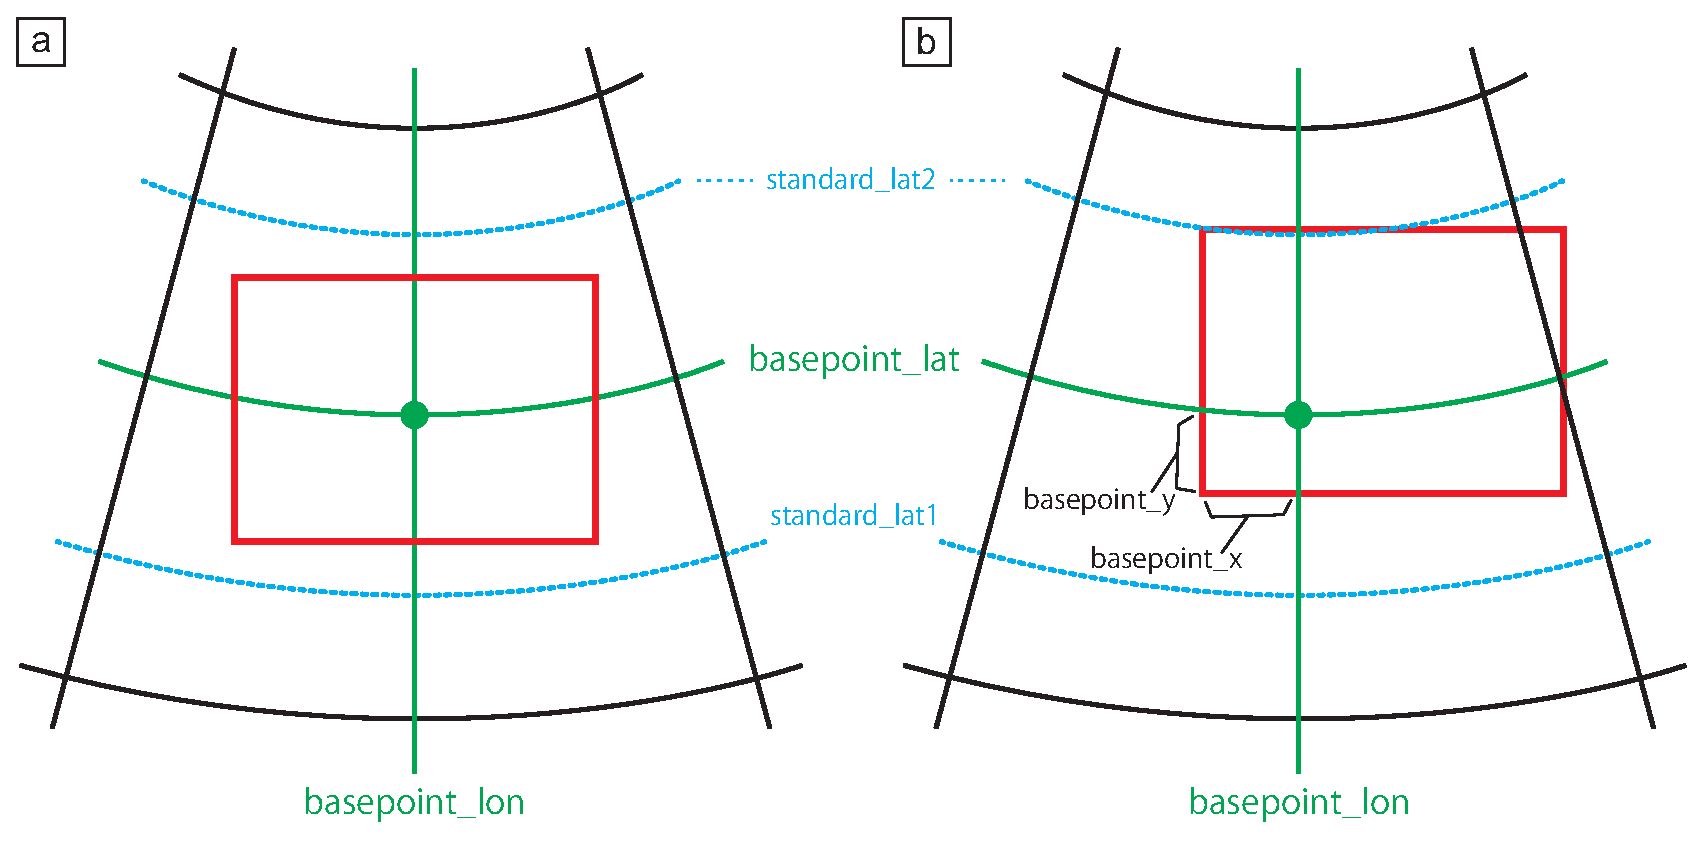
\includegraphics[width=0.8\hsize]{./figure/LC_latlon_xy.eps}\\
  \caption{投影中心と計算領域の関係:(a)はデフォルト設定の場合、(b)は計算領域の位置を投影中心からずらした場合。
  赤線の矩形が計算領域を表す。}
  \label{fig:map_lc}
\end{center}
\end{figure}


\subsection{側面境界条件} \label{sec:adv_lateralbnd}
%------------------------------------------------------
SCALEでは、側面境界条件として「周期境界条件」と「外部入力データ指定」の2種類から選択できる。デフォルトの設定は東西方向、
南北方向ともに周期境界条件となっている。主に理想実験では周期境界条件を使用し、現実大気実験では外部入力データ指定
を使用することを想定している。設定方法によっては、他の側面境界条件も設定可能であるが、現在のところ想定外の
使用方法であるためサポートできない。

側面境界条件の設定は、configファイルの\verb|PARAM_PRC|の項目を編集することで設定できる。
\textcolor{red}{\bf この設定は、pp\_***.conf、init\_***.conf、run\_***.confのconfigファイルの間で
必ず一致させなければならない。} 周期境界条件を設定したい場合は、デフォルト設定なので特にconfigファイルに記述する
必要はない。理想実験チュートリアルのconfigファイルの\verb|PARAM_PRC|の項目を見れば特に境界条件に関する記述が
ないことがわかるだろう。一方、外部入力データ指定を設定したい場合は、下記のように``\verb|PRERIODIC|''のスイッチを
``false''に指定する。\\

\noindent {\small {\gt
\ovalbox{
\begin{tabularx}{140mm}{l}
\verb|&PARAM_PRC| \\
\verb|      〜 中略 〜|\\
\verb| PRC_PERIODIC_X  = .false.,| \\
\verb| PRC_PERIODIC_Y  = .false.,| \\
\verb|/| \\
\end{tabularx}
}}}\\

\noindent 外部入力データ指定の場合は、\ref{sec:adv_gridspace}節で説明した必ず側面境界のバッファー領域を
設定しなければならない。バッファー領域でどの変数に強制をかけるか(ダンピングするか)、またその場合の時定数などの
設定はconfigファイルの\verb|PARAM_ATMOS_BOUNDARY|の項目で指定できる。現実大気実験のチュートリアルの
configファイル(\verb|run.conf|)を元にして一部の項目を説明する。\\

\noindent {\small {\gt
\ovalbox{
\begin{tabularx}{140mm}{l}
\verb|&PARAM_ATMOS_BOUNDARY|\\
\verb| ATMOS_BOUNDARY_TYPE        = "REAL",|\\
\verb| ATMOS_BOUNDARY_IN_BASENAME = "../init/boundary_d01",|\\
\verb| ATMOS_BOUNDARY_USE_VELZ    = .true.,|\\
\verb| ATMOS_BOUNDARY_USE_QHYD    = .false.,|\\
\verb| ATMOS_BOUNDARY_VALUE_VELZ  = 0.0D0,|\\
\verb| ATMOS_BOUNDARY_UPDATE_DT   = 21600.0D0,|\\
\verb|/|\\
\end{tabularx}
}}}\\

上2つの項目は、``REAL''が外部入力データを使用することを意味し、次の行の指定がその外部入力データのファイル名を指定している。
上から3つ目の設定項目である``\verb|ATMOS_BOUNDARY_USE_VELZ = .true.|''は、鉛直速度に対して「強制をかける」ことを
意味している。一方、``\verb|ATMOS_BOUNDARY_USE_QHYD = .false.|''として、凝結物の混合比に対しては逆に「強制をかけない」
設定になっている。その次の項目の``\verb| ATMOS_BOUNDARY_VALUE_VELZ|''は、鉛直速度に対して
強制をかける際、ここで指定した値、``0.0 m/s''へ近づくように強制をかけるという指定を意味する。
最後の行の``\verb|ATMOS_BOUNDARY_UPDATE_DT|''は、外部入力データの更新間隔が21600秒であることを
意味している。たとえば、6時間間隔でデータが与えられている再解析データを外部入力データとして使用する場合にこの設定になる。

他にも、水平速度東西成分(\verb|VELX|)、水平速度南北成分(\verb|VELY|)や温位(\verb|POTT|)などに対して同様の設定項目が
存在する。また、ダンピングの時定数を設定する\verb|ATMOS_BOUNDARY_TAUX|や\verb|ATMOS_BOUNDARY_TAUY|といった設定項目がある。
更なる詳細については、付録\ref{app:namelist}を参照のこと。


%と加える(どちらの変数もデフォルトはtrueで周期境界が用いられる).スポンジ層ではレイリーダンピングがかけられる.
%スポンジ層でかけるレイリーダンピングの設定はrun.confのPARAM\_ATMOS\_BOUNDARYで設定する.
%設定方法の一例とそれぞれのNamelistの意味を下に示す.
%\begin{verbatim}
% ATMOS_BOUNDARY_TYPE         = "INIT",  (初期値に近づくように緩和する)
% ATMOS_BOUNDARY_USE_VELZ     = .true., (速度の鉛直成分にダンピングを適用する)
% ATMOS_BOUNDARY_USE_VELX     = .true., (速度のx成分にダンピングを適用する)
% ATMOS_BOUNDARY_USE_VELY     = .true., (速度のy成分にダンピングを適用する)
% ATMOS_BOUNDARY_USE_POTT     = .true., (温位にダンピングを適用する)
% ATMOS_BOUNDARY_USE_QV       = .true., (温位にダンピングを適用する)
% ATMOS_BOUNDARY_TAUX         =  300.D0, (x方向のダンピングの時定数:300[sec])
% ATMOS_BOUNDARY_TAUY         =  300.D0, (y方向のダンピングの時定数:300[sec])
% ATMOS_BOUNDARY_TAUZ         =  10.D0,  (z方向のダンピングの時定数:300[sec])
%\end{verbatim}
%各Namelistの詳細はAppendixを参照されたい.


\subsection{積分時間と積分時間間隔の設定} \label{sec:adv_timeintiv}
%------------------------------------------------------
例えば理想実験チュートリアルでは、積分時間は1時間とし、時間積分間隔として力学過程は1.0秒、雲物理過程は10.0秒で実行したが、
積分時間を伸ばしたい場合や、計算にかかる時間を短くするために積分時間間隔を長くしたり、計算不安定を防ぐために
積分時間間隔を短くすることがあるだろう。

積分時間と積分時間間隔の設定は、configファイル\verb|run_***.conf|の\verb|PARAM_PRC|の項目を編集することで設定できる。
この項目はモデル本体の実行だけで有効である。理想実験チュートリアルで使用した\verb|run_R20kmDX500m.conf|の例を示す。\\

\noindent {\small {\gt
\ovalbox{
\begin{tabularx}{140mm}{l}
\verb|&PARAM_TIME|\\
\verb| TIME_STARTDATE             = 0000, 1, 1, 0, 0, 0,|(計算開始の日付:放射過程を用いる実験等で必要)\\
\verb| TIME_STARTMS               = 0.D0,| (計算開始時刻[mili sec])\\
\verb| TIME_DURATION              = 3600.0D0,| (積分時間[単位はTIME\_DURATION\_UNITで決定])\\
\verb| TIME_DURATION_UNIT         = "SEC",| (積分時間TIME\_DURATIONの単位)\\
\verb| TIME_DT                    = 5.0D0,| (移流のタイムステップ)\\
\verb| TIME_DT_UNIT               = "SEC",| (TIME\_DTの単位)\\
\verb| TIME_DT_ATMOS_DYN          = 1.0D0,| (力学過程のタイムステップ)\\
\verb| TIME_DT_ATMOS_DYN_UNIT     = "SEC",| (TIME\_DT\_ATMOS\_DYNの単位)\\
\verb| TIME_DT_ATMOS_PHY_MP       = 10.0D0,| (雲物理過程のタイムステップ)\\
\verb| TIME_DT_ATMOS_PHY_MP_UNIT  = "SEC",| (TIME\_DT\_ATMOS\_PHY\_MPの単位)\\
\verb|/|\\
\end{tabularx}
}}}\\

上記の各部分を変更することで積分時間や積分時間間隔を変更することができる。


\section{物理モデルの利用} \label{sec:adv_physics}
%------------------------------------------------------
本節では雲物理モデルや乱流モデルなどの物理モデルの利用方法を説明する。
チュートリアル実験で用いてきた物理モデルについて理解するためにconfigファイルの設定を再確認しながら説明をすすめる。
ここでは例として、理想実験チュートリアルのsampleディレクトリ内にある\verb|run_R20kmx20kmDX500m.conf|を取り上げる。


\subsection{雲微物理スキームの設定} \label{sec:adv_microphys}
%------------------------------------------------------
チュートリアルでは、\cite{tomita_2008}の1-momentバルク法を用いていたが、SCALEには暖かい雲のみを考慮する1-momentバルク法
(\cite{kessler_1969}),氷雲を含んだ2-momentバルク法(\cite{sn_2014})、1-momentビン法の4種類の雲微物理スキーム
(\cite{suzuki_etal_2010})も利用することが可能である。
これらの雲微物理スキームの選択は,init.confとrun.confに記載されているPARAM\_TRACERに含まれる
``TRACER\_TYPE''及び,PARAM\_ATMOSに含まれる``ATMOS\_PHY\_MP\_TYPE''によって設定する。
{\bf 両者は同じにする必要があり},選択する雲微物理スキームによって以下のように設定する。

\begin{verbatim}
KESSLER :水雲のみの1-momentバルク法(Kessler 1969)
TOMITA08:氷雲を含む1-momentバルク法(Tomita 2008)
SN14    :氷雲を含む2-momentバルク法(Seiki and Nakajima 2014)
SUZUKI10:1-momentビン法(Suzuki et al. 2010,氷雲を含むか否かはオプションで選択)
\end{verbatim}

このとき\textcolor{red}{TRACER\_TYPEとATMOS\_PHY\_MP\_TYPEはinit.conf,run.confで同一にする必要がある}ことに注意されたい.
SUZUKI10以外を選択した場合は、init.conf、run.confのTRACER\_TYPEとATMOS\_PHY\_MP\_TYPEを変更するだけで実行可能である。
一方SUZUKI10を選択した場合は、init.conf、run.confの双方に\\

\noindent {\small {\gt
\ovalbox{
\begin{tabularx}{140mm}{l}
\verb|&PARAM_BIN| \\
\verb| nbin   = 33, (ビンの数)| \\
\verb| ICEFLG =  1, (氷雲を考慮するか否か,0->水雲のみ,1->氷雲も含む)| \\
\verb|/| \\
\end{tabularx}
}}}\\

を追記し、さらにinit.confに記載されているPARAM\_MKINITに「flg\_bin = .true. 」を追加する必要がある。\\

\noindent {\small {\gt
\ovalbox{
\begin{tabularx}{140mm}{l}
\verb|&PARAM_MKINIT| \\
\verb|     〜 中略 〜|\\
\verb| flg_bin = .true.| \\
\verb|     〜 中略 〜|\\
\verb|/| \\
\end{tabularx}
}}}\\

この場合も、{\bf init.confとrun.confに記載されるPARAM\_BINは同一にする必要がある}。
SUZUKI10を選択した時には、micpara.datという
雲微物理の計算に必要なファイルが自動生成される。micpara.datがすでに存在する場合は存在する場合はあるものを利用するが、
nbinが変わると新たに作成しなければならない。micpara.datにnbinの情報が記載されているが、もしrun.confに記載されるnbinと
micpara.datに記載されているnbinが異なれば、\\

\noindent {\gt
\fbox{
\begin{tabularx}{140mm}{l}
\verb|xxx nbin in inc_tracer and nbin in micpara.dat is different check!| \\
\end{tabularx}
}}\\

\noindent というエラーメッセージを標準出力に出力して計算が落ちるようになっている。
そのため、nbinを変更した際は、micpara.datを消去して
新たに作り直す必要がある(micpara.datを消して再度SCALEをSUZUKI10を用いて実行すれば自動的に新しいmicpara.datが生成される)。


\subsection{乱流スキームの設定} \label{sec:adv_turbulence}
%------------------------------------------------------
理想実験チュートリアルでは乱流スキームは導入されていなかったが、SCALEにはSmagorinsky typeの乱流スキーム
(\cite{smagorinsky_1963}; \cite{lilly_1962}; Brown 1994; Scotti et al. 1994)とMellor-Yamada Level 3の
乱流スキーム(MYNN, \cite{my_1982},\cite{nakanishi_2004})導入されている。
これらを利用するには,init.confとrun.conf双方のPARAM\_ATMOSに「ATMOS\_PHY\_TB\_TYPE」を加える。

\begin{verbatim}
ATMOS_PHY_TB_TYPE="SMAGORINSKY" (Smagorinsky typeのサブグリッドモデル)
ATMOS_PHY_TB_TYPE="MYNN" (Mellor-Yamada Level 3のRANSモデル)
\end{verbatim}

またrun.confのPARAM\_TIMEに

\begin{verbatim}
 TIME_DT_ATMOS_PHY_TB       = 0.10D0,  (乱流スキームの時間ステップ)
 TIME_DT_ATMOS_PHY_TB_UNIT  = "SEC", (TIME_DT_ATMOS_PHY_TBの単位)
\end{verbatim}

を加える。これらを設定した上で,run.shを実行することで,乱流スキームを考慮した計算が可能になる.
地表面フラックスのバルク係数を決めるスキーム,放射スキーム,都市スキームなどに関しては,
現実事例を対象とした4章を参照されたい.


\subsection{放射過程の設定} \label{sec:adv_radiation}
%------------------------------------------------------
SCALEには、放射過程としてMSTRN (\cite{sekiguchi_2008})が実装されている。ここでは、MSTRNの設定方法を説明する。

放射モデルを実行するには、各種外部データとパラメタテーブルが必要である。
オゾンのプロファイルなどの外部データとパラメタテーブルは、``scale-rm/test/data/rad/''の中に与えられている。
放射過程を利用する実験を行う場合は、必ず``scale-rm/test/data/rad/''下の外部データとパラメタテーブルが必要である。
詳細に関しては随時説明を加えていく。


\subsection{陸面・海洋上の地表面フラックスモデルの設定} \label{sec:adv_landocean}
%------------------------------------------------------
SCALEには、陸面モデルとしてバケツモデル(バルク交換係数は \cite{beljaars_1991}; \cite{wilson_2001}に基づく)が
実装されている。また海洋上のフラックスモデルとしてスラブモデルが実装されている。
ここでは、陸面モデルと海洋モデルの設定方法について説明する。

陸面モデルを実行するには、土地利用データとそれに対応するパラメタテーブルが必要である。
パラメタテーブルは、``scale-rm/test/data/land/''の中に``param.bucket.conf''というファイルで与えられている。
中には10種類を超える土地利用区分とそれらに対応する粗度長などのパラメタが与えられている。陸面が存在する領域で実験
を行う場合は、必ず``param.bucket.conf''のパラメタテーブルが必要である。
詳細に関しては随時説明を加えていく。


\subsection{都市モデルの設定} \label{sec:adv_urban}
%------------------------------------------------------
SCALEには、都市モデルとして単層キャノピーモデル(\cite{kusaka_2001})が実装されている。
ここでは都市モデルの設定方法について説明する。
詳細に関しては随時説明を加えていく。


\section{任意のデータをSCALEで使用する} \label{sec:adv_datainput}
%====================================================================================

%\subsection{Topography and Landuse}

%現在のSCALEでは用意されている地形・土地利用データよりも
%高い解像度での計算ができない。
%高解像度計算のためには、ユーザーが適宜データを用意する必要がある。

%scale-rmでは日本領域については国土地理院のデータをもとにした地形,土地利用に関するデータベースを別途提供している(2.2節を参照).


\subsection{初期値・境界値データ} \label{sec:adv_bnddata}
%------------------------------------------------------
現在、SCALEでは下記のデータの読み込みとそれらに基づく初期値・境界値作成に対応している。

\begin{table}[htb]
\begin{center}
\caption{SCALEが読込に対応する外部入力データフォーマット}
\begin{tabularx}{150mm}{|l|l|l|X|} \hline
 \rowcolor[gray]{0.9} データ形式 & 対応状況 & \verb|FILETYPE_ORG| & 備考 \\ \hline
 バイナリデータ & \textcolor{blue}{対応} & \verb|GrADS| & データ読み込み用のnamelistを別途必要とする。 \\ \hline
 NICAMデータ & \textcolor{blue}{対応} & \verb|NICAM-NETCDF| & netCDF形式のLatLonデータに対応する。 \\ \hline
 WRFデータ & \textcolor{blue}{対応} & \verb|WRF-ARW| & ``wrfout''、``wrfrst''の両方に対応する。 \\ \hline
 SCALEデータ & \textcolor{blue}{対応} & \verb|SCALE-RM| & historyデータのみ対応;latlonカタログを必要とする。 \\ \hline
\end{tabularx}
\label{tab:inputdata_format}
\end{center}
\end{table}

これらの使い分けは、初期値・境界値作成時、すなわち``scale-rm\_init''の実行時のconfigファイルの
\verb|PARAM_MKINIT_REAL|の項目中の\verb|FILETYPE_ORG|に表\ref{tab:inputdata_format}に示した設定値を
指定することで使い分ける。

最も汎用的に使用するデータ形式は「バイナリデータ」になることと思う。ここでいうバイナリデータとは、「4バイト単精度
浮動小数点のダイレクトアクセス方式、Fortran型バイナリデータ」を指す。その主な使用方法は、
第\ref{sec:tuto_real}章の現実大気実験チュートリアルで説明したとおりである。\textcolor{red}{GRIB/GRIB2のデータ形式は、
チュートリアルで説明した方法に基づいて、バイナリデータ形式を経由してSCALEに読み込ませることができる。}
その他に任意のデータを境界値に使用したい場合は、バイナリデータ形式に変換することで読み込ませることができる。

SCALEデータ形式は主にオフライン・ネスティング実験で使用される。詳細については、\ref{sec:nest_offline}節を
参照されたい。NICAMデータ形式は、nativeのicosahedral grid systemデータではなく、緯度・経度座標に変換されたデータの
み読み込みに対応している。WRFデータ形式についてはモデル出力データをそのまま使用することができる。
これらの読み込み方法に関しては随時説明を加えていく。





%%%%%%%%%%%%%%%%%%%%%%%%%%%%%%%%%%%%%%%%%%%%%%%%%%%%%%%%%%%%%%%%%%%%%%%%%%%%%%%%%%%%%%
